\documentclass[8pt]{beamer}

\usepackage[utf8x]{inputenc}
\usepackage{default}

\usepackage[T1]{fontenc}
\usepackage[spanish]{babel}
\usepackage{amsmath,amsfonts,amsthm}

\usepackage{pgfplots}
\pgfplotsset{compat=1.15}

\usepackage{mathtools}
\usepackage{tikz}
\tikzstyle{every picture}+=[remember picture]
\setbeamertemplate{enumerate items}[square]

\setbeamertemplate{footline}{\insertframenumber/\inserttotalframenumber}

%    NUEVOS COMANDOS DEFINIDOS MEDIANTE NEWCOMAND
\DeclareMathOperator\erf{erf}

% ENTORNO MATEMÁTICO
\newcommand{\maths}[1]{$ #1 $}

% TEXTO RESALTADO
\newcommand{\resalta}[1]{\textit{#1}}
\newcommand{\anglicismo}[1]{\textit{#1}}
\newcommand{\cultismo}[1]{\textit{#1}}
\newcommand{\comillas}[1]{``#1''}

% SÍMBOLOS MATEMÁTICOS
\newcommand{\menoroigual}{$\geqslant$}
\newcommand{\delorden}{$\sim$}
\newcommand\norm[1]{\left\lVert#1\right\rVert}
\newcommand{\porcentaje}[1]{$#1\:\%$}

\newcommand{\gonzalez}{González-Nuevo et al.}
\newcommand{\negrello}{Negrello et al.}


% UNIDADES
%   PROPIAS DE ASTRONOMÍA
\newcommand{\solares}[2]{$#2 \:{#1}_{\odot}$}
\newcommand{\masassolares}[1]{$#1 \:{M}_{\odot}$}
\newcommand{\luminosidadessolares}[1]{$#1 \:{L}_{\odot}$}
\newcommand{\tfe}[1]{$#1 \:{M}_{\odot}\,\mathrm{{yr}^{-1}}$}
% \newcommand{\myr}{}
\newcommand{\flujo}[1]{${S}_{#1 \:\mu\mathrm{m}}$}
%   GENERALES
\newcommand{\microm}[1]{$#1 \:\mu\mathrm{m}$}
\newcommand{\angstrom}[1]{$#1 \:$\AA}
\newcommand{\mjy}[1]{$#1 \:\mathrm{mJy}$}
\newcommand{\jy}[1]{$#1 \:\mathrm{Jy}$}
\newcommand{\kelvin}[1]{$#1 \:\mathrm{K}$}
%   Grados celsius
\newcommand{\celsius}{\hspace{-2,5mm}$\phantom{a}^{\circ} \mathrm{C}$~}
\newcommand{\grad}{$^{\circ}$}

% NOMBRES USADOS FRECUENTEMENTE
\newcommand{\hatlas}{\mbox{\textit{H}-ATLAS}}
\newcommand{\halos}{\mbox{HALOS}}
\newcommand{\halo}{\mbox{HALO}}
\newcommand{\gama}{\mbox{GAMA}}
\newcommand{\spire}{\mbox{SPIRE}}
\newcommand{\pacs}{\mbox{PACS}}
\newcommand{\hifi}{\mbox{HIFI}}
\newcommand{\h}{\textit{\mbox{Herschel}}}
\newcommand{\rt}{\textit{\mbox{redshift}}}
\newcommand{\rts}{\textit{\mbox{redshifts}}}
\newcommand{\sed}{\mbox{SED}}
\newcommand{\sfr}{\mbox{SFR}}
\newcommand{\slg}{\mbox{SLG}}
\newcommand{\etg}{\mbox{ETG}}
\newcommand{\cross}{\mbox{cross-identificación}}
\newcommand{\smm}{\mbox{SMM~J2135-0102}}
\newcommand{\arp}{\mbox{Arp220}}
\newcommand{\gquince}{\mbox{G15.141}}
\newcommand{\typewriter}[1]{\texttt{#1}}
\newcommand{\python}{\texttt{\mbox{Python}}}


\newcommand{\paramk}{'K'}
\newcommand{\paramc}{'C'}

  
  
  
  

\begin{document}


%Transparencia 1 Titulo,fecha,nombre.
\begin{frame}
\title{Selección de fuentes extragalácticas a alto \rt\ mediante una herramienta estadística de
\cross\ de catálogos de galaxias.}
\author{Javier Gutiérrez Solórzano}
\date{Febrero 2018}

\maketitle

\end{frame}


%Transparencia 2
\begin{frame}
\frametitle{Contenidos}

\begin{itemize}
\item \large {Estado del arte y objetivos.}
\item \large {Método de Cross-identificación.}
\item \large {Método para estimar el \rt\ fotométrico de las ETGs.}

\item \large {Resultados.}

\item \large {Conclusiones.}

\end{itemize}

\end{frame}


%Transparencia 3
\begin{frame}

\frametitle{Estado del arte}

\begin{itemize}

\item Objetos con alto \rt, en su mayoría ETGs (Early Type Galaxies).

Características
\maths{
 \begin{cases}
 
    \text{Se encuentran muy lejos $\implies$ Son muy débiles} \\
    
    \text{Máximo de emisión en IR-lejano (\microm{50-500})}\\
 \end{cases}
}

La actual generación de telescopios IR tiene una resolución angular baja para estudiar este típo de objetos \maths{\implies} hace de las ETGs objetos difíciles de observar directamente.

\item Lentes gravitatorias producen magnificaciones que facilitan el estudio de las ETGs $\implies$ Interés en el desarrollo de criterios para identificar SLGs (Strong lensing galaxies); utilizan argumentos físicos basados en nuestro conocimiento actual de las ETGs.

\item Dos criterios \maths{
 \begin{cases}
 
    \text{\negrello} \\
    
    \text{\gonzalez}\\
 \end{cases}
}

Ambos proponen uno o varios límites de densidades de flujo espectral a longitudes de onda concretas por encima de las cuales se espera que las galaxias submilimétricas hayan
sido lensadas (magnificadas por efecto lente gravitatoria).

\end{itemize}

\end{frame}


%Transparencia 4
\begin{frame}{Objetivos}

Objetivos

\begin{itemize}

\item Hacer una propuesta complementaria a los métodos de identificación de SLGs ya existentes.

\item Se van a buscar sistemas lente gravitatoria completos (fuentes y lentes del sistema lente gravitatoria en catálogos diferentes).

\end{itemize}

¿Cómo pretendemos alcanzar los objetivos?  
 
\begin{itemize}

\item Se va a utilizar un criterio puramente estadístico basado en dos factores de Bayes.

\item Seleccionando un subconjunto de emparejados que surgen al aplicar un método de cross-identificación de catálogos de galaxias, a los catálogos \hatlas\ DR1 y \gama\ DR1.

\end{itemize}
    
\end{frame}


%Transparencia 5
\begin{frame}
\frametitle{¿Por qué estos catálogos?}

\hatlas\ (fuentes)

\begin{itemize}
    \item \hatlas\ se fundamenta en las medida del telescopio espacial \h\ que es sensible a las longitudes de onda en el IR-lejano donde se encuentra el máximo de emisión de las ETGs.
    
    \item Se estima que la sección eficaz de detección de lentes a alto \rt\ por el instrumento \spire\ es muy favorable (alto \rt\ \maths{\implies} \maths{z>1})
    
\end{itemize}

\vspace{.5cm}

\gama\ (lente)

\begin{itemize}
    \item El catálogo \gama\ DR1 tiene un área de solapamiento con el catálogo \hatlas\ DR1.
    
    \item El proyecto tiene por objetivo estudiar el universo cercano (\rt\ bajo e intermedio, \maths{z<1}).
    
\end{itemize}

\end{frame}


%Transparencia 6
\begin{frame}

\frametitle{Método de cross-identificación}

Formamos emparejados formados por dos observaciones pertenecientes a dos catálogos diferentes y les asignamos dos factores de Bayes diferentes.

\vspace{2mm}

El factor de Bayes se define como el cociente de la función verosimilitud de dos hipótesis alternativas

\begin{equation*}
    B_{12}=\frac{p(D|H_1)}{p(D|H_2)},
\end{equation*}

donde los subíndices hacen referencia a la hipótesis 1 y 2 respectivamente.


\begin{itemize}

    \item \maths{H_1} la hipótesis de que los emparejados considerados están formados por observaciones de un mismo objeto astronómico.
    
    \item \maths{H_2} la hipótesis de que se trata de observaciones pertenecientes a dos objetos diferentes.
    
\end{itemize}
Los dos factores de Bayes utilizados han sido propuestos por T. Budavári y A. S. Szalay.

\end{frame}


%Transparencia 7
\begin{frame}

\frametitle{Método de cross-identificación}

Los factores de Bayes son:

\begin{itemize}

\item Factor de Bayes posicional:

\begin{equation*}
    B_{12}^{p}= \frac{2}{{\sigma}^2_1+{\sigma}^2_2}\exp{\left(- \frac{{\phi}^{2}_{12}}{2({\sigma}^2_1+{\sigma}^2_2)} \right)}
\end{equation*}

\hspace{2mm}

\maths{\sigma_1} y \maths{\sigma_2} desviación típica asociada al error posicional.

    \begin{itemize}
         \item Depende de la separación angular (\maths{{\phi}_{12}}) entre las observaciones.
    \end{itemize}    

\hspace{2mm}

\item Factor de Bayes fotométrico:

\small{

\begin{equation*}
    \hspace{-5mm} B_{12}^{z}=\frac{\sqrt{2}\:z_{max}\exp{\left(-\frac{{(z_1-z_2)}^{2}}{2({\sigma}_{1}^{2}+{\sigma}_{2}^{2})}\right)}\left[ \erf{\left( \frac{{\sigma}_{1}^{2}z_2+{\sigma}_{2}^{2}z_1}{\sqrt{2}\sigma_1\sigma_2\sqrt{\sigma_1^2+\sigma_2^2}}  \right)}- \erf{\left( \frac{{\sigma}_{1}^{2}(z_2-z_{max})+\sigma_2^2(z_1-z_{max})}{\sqrt{2}\sigma_1\sigma_2\sqrt{\sigma_1^2+\sigma_2^2}}  \right)} \right]}{\sqrt{\pi(\sigma_1^2+\sigma_2^2)}\left[\erf{\left(\frac{z_1}{\sqrt{2}\sigma_1}\right)}-\erf{\left(\frac{z_1-z_{max}}{\sqrt{2}\sigma_1}\right)}\right]\left[\erf{\left(\frac{z_2}{\sqrt{2}\sigma_2} \right)}-\erf{\left(\frac{z_2-z_{max}}{\sqrt{2}\sigma_2} \right)}\right]}
\end{equation*}

}

\normalsize

\hspace{2mm}

\maths{\sigma_1} y \maths{\sigma_2} desviación típica relativa a los valores del \rt.

\begin{itemize}
    \item Depende de la diferencia entre \rts\ de las observaciones. 
\end{itemize} 

\end{itemize} 

\end{frame}


%Transparencia 8
\begin{frame}

\frametitle{Método de cross-identificación}

Factor de Bayes conjunto:

\begin{equation*}
    B_{12}= B^{p}_{12}\times B^{z}_{12}
\end{equation*}

Criterio:

\begin{itemize}

\item En el caso de que el factor de Bayes \maths{B_{12}>1} la función verosimilitud de \maths{H_1} es mayor que la verosimilitud de la hipótesis \maths{H_2} \maths{\implies} Las observaciones pertenecen al mismo objeto.

\item En el caso de que el factor de Bayes \maths{B_{12}<1} la función verosimilitud de \maths{H_2} es mayor que la verosimilitud de la hipótesis \maths{H_1} \maths{\implies} Las observaciones pertenecen a objetos diferentes.
 
\end{itemize}

Para el obtener el factor de Bayes fotométrico:

\begin{itemize}
    \item \hspace{.1cm} Problema: La mayoría de las fuentes de \hatlas\ y \gama\ no disponen de una medida de su \rt.
    
    \item \hspace{.1cm} Solución: Si la fuente pertenece a \hatlas\ hemos utilizado un método propuesto por \gonzalez\ para estimar dicho valor a partir de las medidas de \spire.
    
\end{itemize}
    
\end{frame}


%Transparencia 9
\begin{frame}

\frametitle{Método para estimar el \rt\ fotométrico de las ETGs a partir de \spire}

¿En qué consiste el método?

Se realiza un ajuste por mínimos cuadrados de la SED normalizada de la galaxia modelo \smm\ a tres medidas proporcionadas por el instrumento \spire.

\begin{itemize}

\item ¿Por qué funciona?
Porque las medidas de \spire\ se encuentran el la zona donde la SED de la ETGs se modela mediante la suma de dos cuerpos grises. (para la galaxia \smm\ dos cuerpos grises con temperaturas de \maths{\mathrm{T}=30\:\mathrm{K}} y \maths{\mathrm{T}=60\:\mathrm{K}} y índices de emisividad \maths{\beta=1.7} y \maths{\beta=2} respectivamente)


\item ¿Por qué la SED de la galaxia \smm? Se realizaron varios estudios que concluyeron que era la SED más adecuada para realizar los ajustes.

\item La SED de las ETGs modelos disponibles no son completamente experimentales. Se dispone de unos pocos puntos y después a partir de modelos teóricos se obtiene el resto e la curva (código GRASIL).

\end{itemize} 

\end{frame}


%Transparencia 10
\begin{frame}

\frametitle{Método para estimar el \rt\ fotométrico de las ETGs a partir de \spire}

\vspace{2mm}

La curva de ajuste se obtiene al multiplicar los valores del flujo por \paramc y los valores de la longitud de onda por \paramk. Para \microm{\lambda \sim 50-500} (sistema en reposo, curva azul) se modela la SED mediante la suma de dos cuerpos grises.

\begin{figure}[htb]
\centering
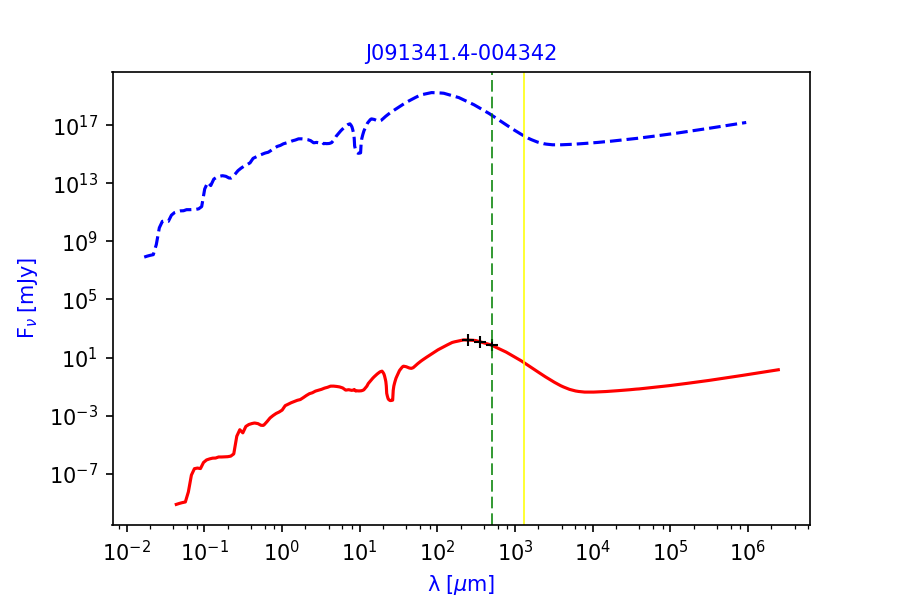
\includegraphics[scale=0.55]{ajuste_6.png}
\end{figure} 

\begin{equation*}
 {\lambda}_{o}={\lambda}_{e}\times K \implies z = \frac{{\lambda}_{o} - {\lambda}_{e}}{{\lambda}_{e}} = \frac{{\lambda}_{o} - \frac{{\lambda}_{o}}{K} }{ \frac{{\lambda}_{o}}{K} } = \frac{ ({\lambda}_{o} \times K) - {\lambda}_{o}}{{\lambda}_{o}} = K - 1.
\end{equation*}

\end{frame}


%Transparencia 11
\begin{frame}

\frametitle{Confrontación del método}

Comparación entre los valores obtenidos utilizando nuestro programa (\maths{z_{\mathrm{phot}}}) y que se encuentran en el artículo de \gonzalez\ (\maths{z_{H}}) para un conjunto de 64 ETGs.

\vspace{-3mm}

\begin{figure}[htb]
\centering
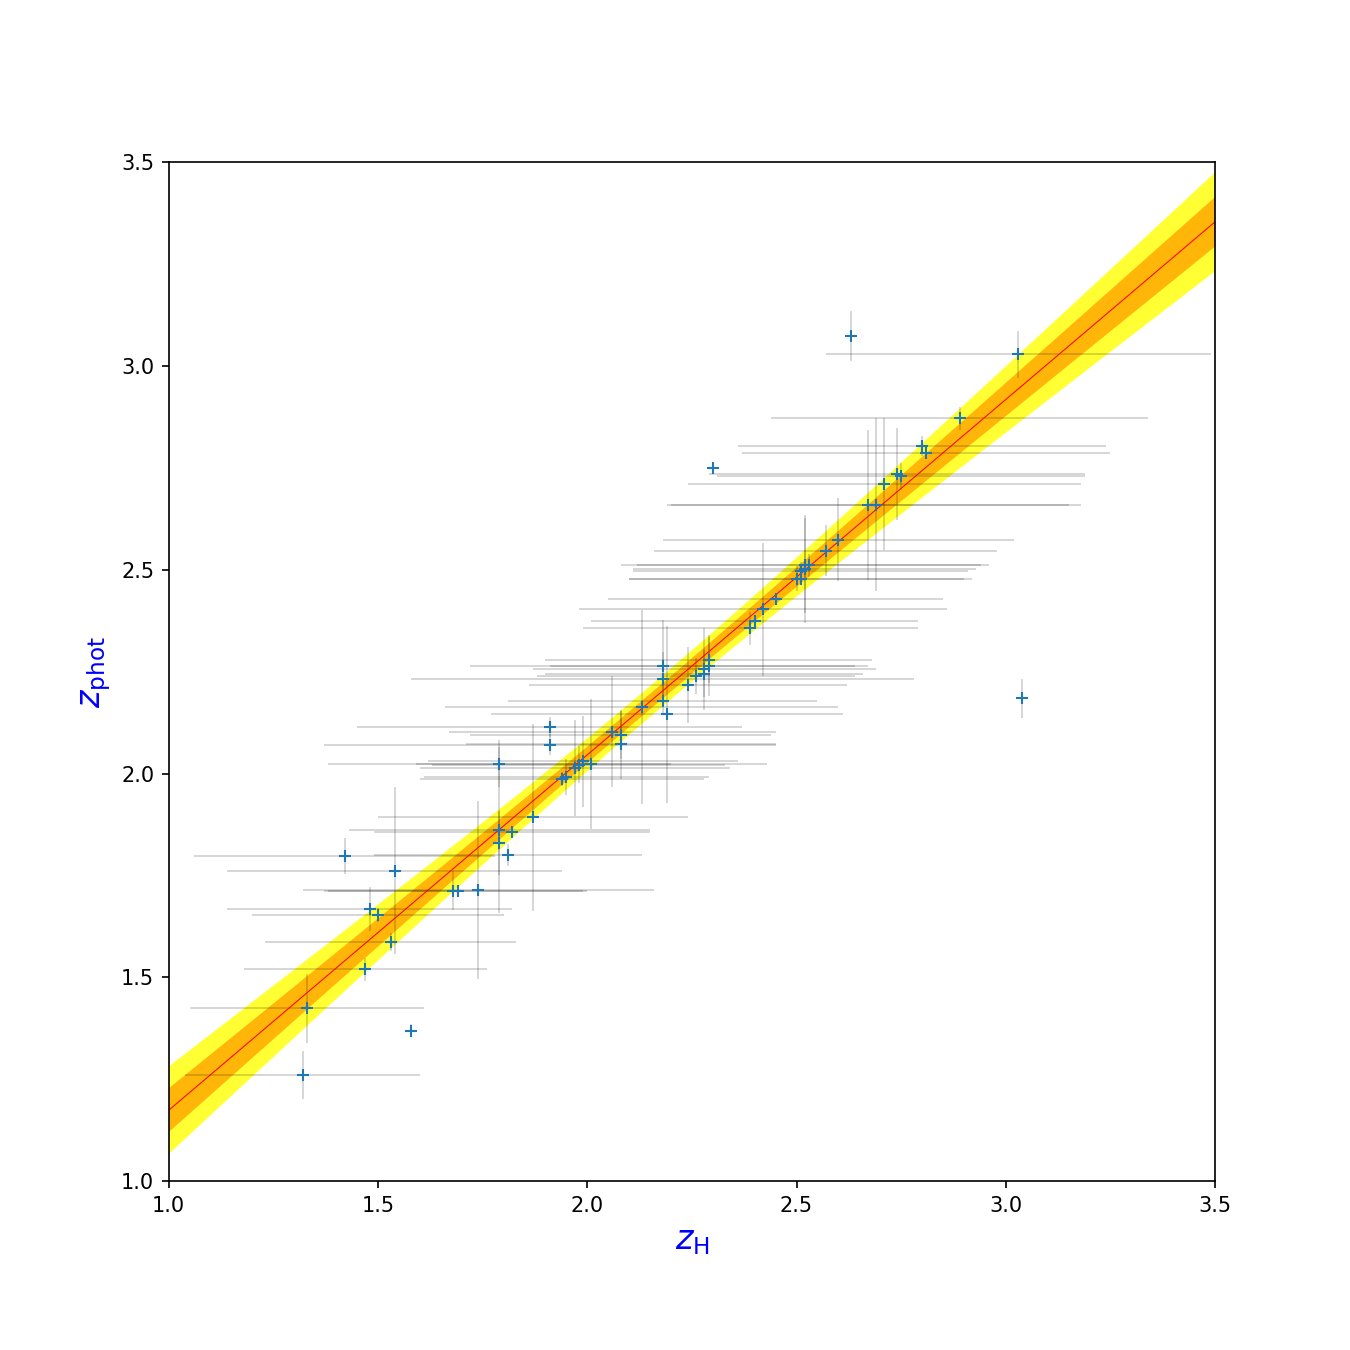
\includegraphics[scale=0.3]{comparacion_Z.png}\par
%\caption{\small Onda cuadrada periódica impar.}
\label{anarmonica}
\end{figure} 

\vspace{-3mm}

\hspace{2.9cm}\maths{{z}_{\mathrm{phot}}=(0.87 \pm 0.04)\times {z}_{\mathrm{H}}+(0.3 \pm 0.1)}

\end{frame}

%Transparencia 12
\begin{frame}

\frametitle{Resumen}

Tenemos:

\begin{itemize}
    
    \item Método de cross-identificación.
    
    \item Método para estimar el \rt\ de las ETGs a partir de las medidas del instrumento \spire.
    
\end{itemize}

¿Cómo usamos todo esto para encontrar lentes gravitatorias?


\end{frame}


%Transparencia 13
\begin{frame}

\frametitle{Nuestra propuesta propuesta.}

Sabemos:

\begin{itemize}
     
\item La separación angular entre los elementos que forman la gravitatoria (la fuente y la lente) es inferior a los \maths{\sim20\:\mathrm{arcsec}} para cuando participan ETGs (la máxima magnificación se produce para el valor del radio de Einstein).

\item Todos los emparejados que tienen una separación angular \maths{{\phi}_{12}<50\:\mathrm{arcsec}} tienen un \maths{B^{p}_{12}>1} (debido a los errores posicionales de los dos catálogos).

\end{itemize}

\vspace{3mm}

Nuestro criterio:

\begin{itemize}
\item Esperamos encontrar lentes gravitatorias dentro del conjunto de emparejados con \maths{B^{p}_{12}>1} y \maths{B_{12}<1} está formado por observaciones que dada su proximidad angular podrían pertenecer al mismo objeto (\maths{{\phi}_{12}<50\:\mathrm{arcsec}}), pero no pueden pertenecer al mismo objeto porque \maths{B_{12}<1}.

\item Si se cumplen las condiciones: \maths{B^{p}_{12}>1}, \maths{B_{12}<1}, \maths{z_h>1} y \maths{z_h>z_g} \maths{\implies} Emparejado candidato a sistema lente gravitatoria.

\end{itemize}

\end{frame}


%Transparencia 14
\begin{frame}{Resultados}

\vspace{-5mm}

\begin{figure}[htb]
\centering
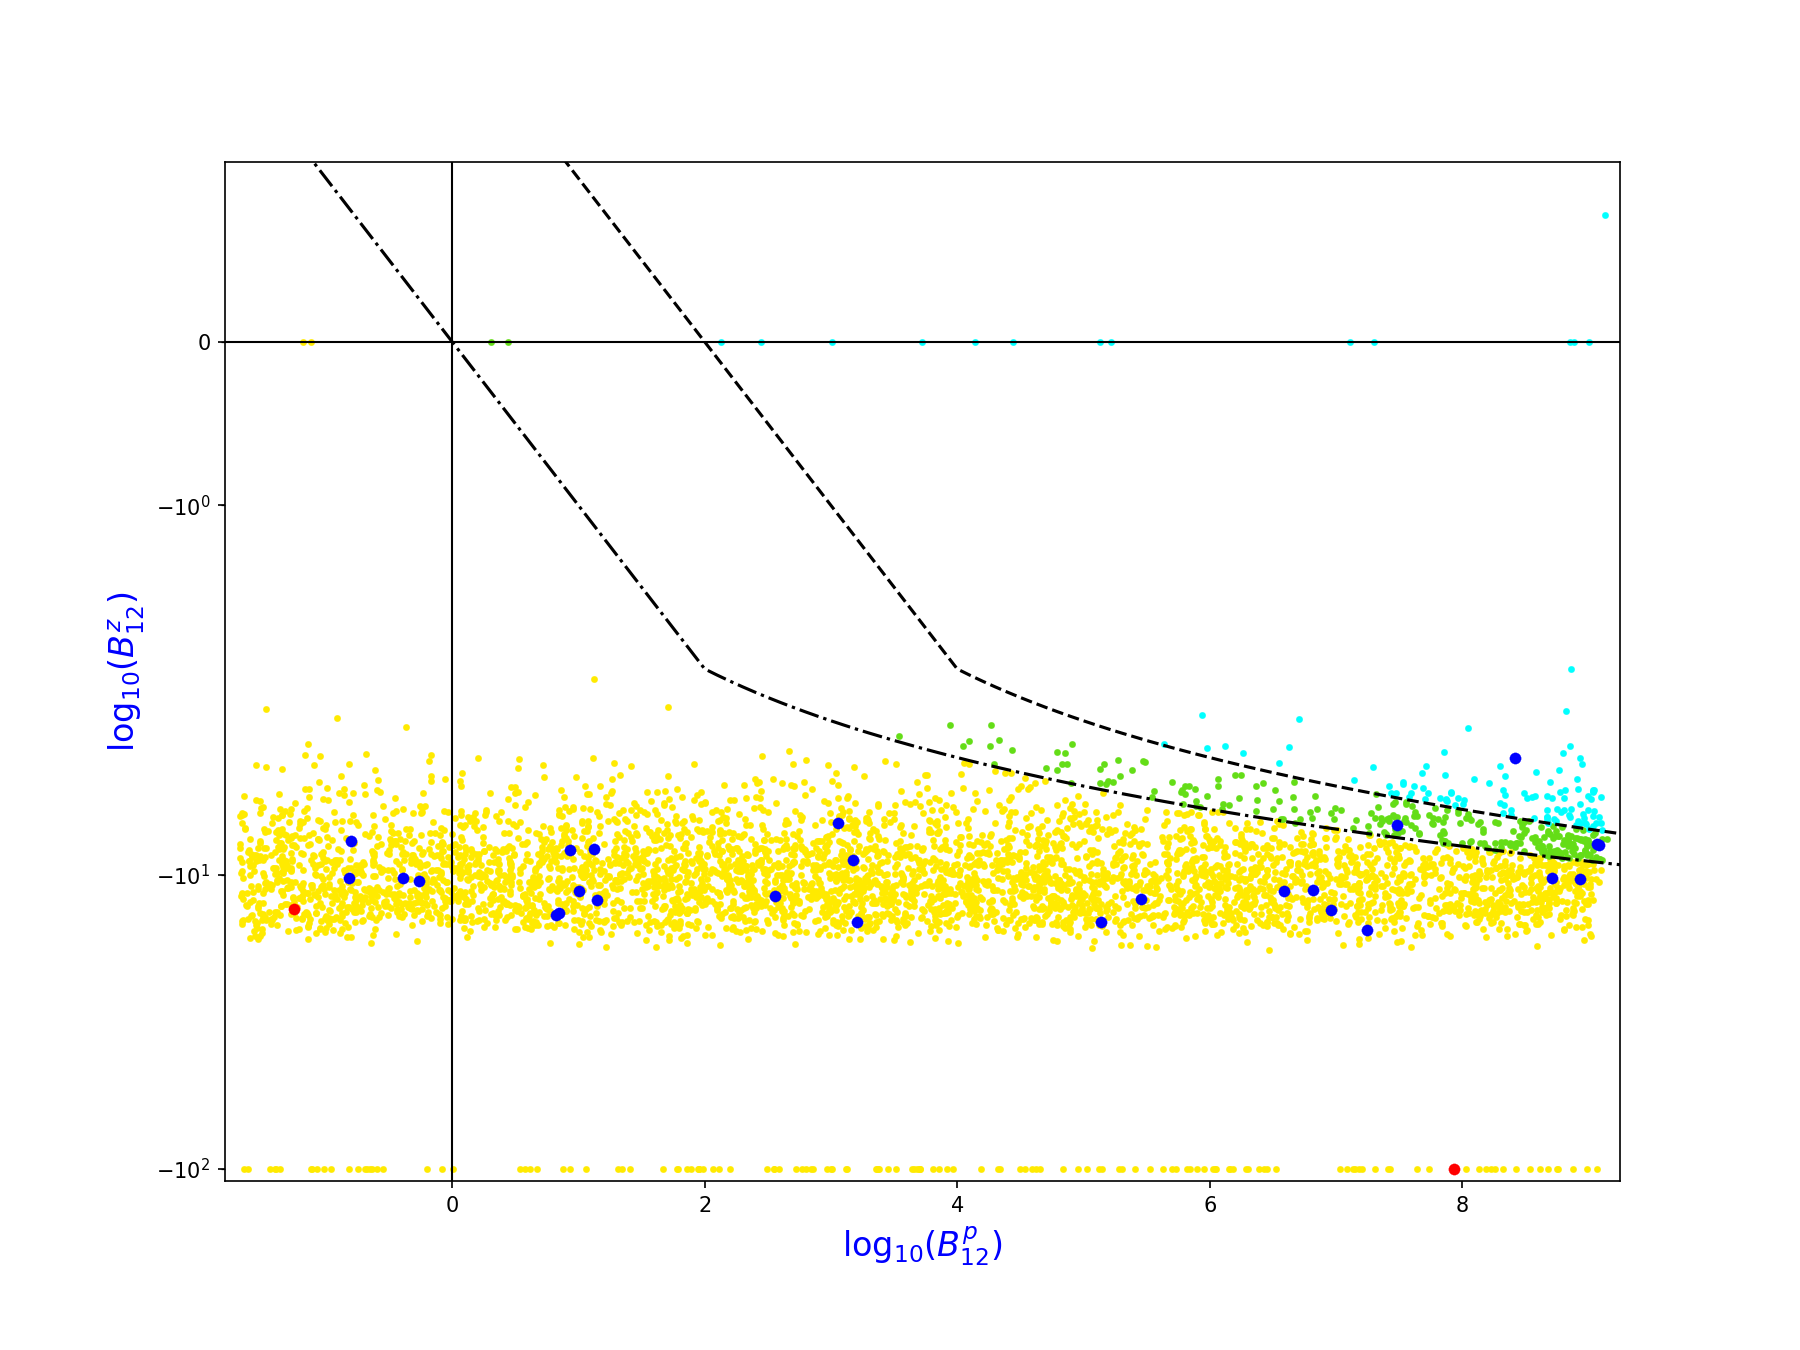
\includegraphics[scale=0.3]{matching_ghfactor_bayes_log_semilog.png}\par
%\caption{\small Onda cuadrada periódica impar.}
\end{figure} 

\vspace{-5mm}
\begin{itemize}
    \item \small{4938 emparejados que cumplen \maths{z_{h}\;>\,1}, \maths{z_{h}>z_{g}} y \maths{\phi<54\;\mathrm{arcsec}}.}
    
    \item 3824 Cumplen además \maths{B^{p}_{12}>1}, \maths{B_{12}<1}.
\end{itemize}

\end{frame}


%Transparencia 15
\begin{frame}{Resultados}

\begin{itemize}

    \item Se han realizado 1000 simulaciones en la que se asignaba a cada observación una posición aleatoria sobre una región con el mismo área que la región original se han encontrado \maths{3521\pm58}.
    
    \item Se han encontrado 3824 emparejados que cumplen nuestras condiciones para ser candidatos a sistema lente gravitatoria en la muestra real.
    
\end{itemize}

- En torno a \maths{\sim200-300} emparejados no pueden ser explicados una distribución aleatoria de las observaciones.

- El número de candidatos en este caso es muy superior al número de candidatos predicho por los otros métodos.

\end{frame}


%Transparencia 16
\begin{frame}{Discusión}

\begin{itemize}
    \item Hay muchos emparejados formados entre observaciones que no guardan relación entre sí (quizás debido a que el radio de emparejamiento es mayor que la distancia entre los elementos que forman las lentes).
    \item El exceso de candidatos que encontramos en la muestra real frente a las muestras simuladas podría explicarse por:
    \begin{itemize}
        \item Lentes gravitatorias.
        \item Debido a una estimación del \rt\ incorrecta, podríamos estar considerando como candidatos a lente gravitatoria emparejados formados por observaciones que en realidad pertenecen al mismo objeto.
    \end{itemize}
    Mejoras propuestas (requieren de conocer con mayor profundidad el fenómeno de las lentes gravitatorias y las ETGs):
    \begin{itemize}
        \item Proponer nuevos factores de Bayes.
        \item Mejorar las funciones densidad de \resalta{probabilidad a priori}.
        \item Mejora del modelo de precisión astrométrica.
        \item Telescopio con mejor resolución angular.
    \end{itemize}
\end{itemize}

\end{frame}


%Transparencia 17
\begin{frame}{Conclusiones}
\begin{itemize}
    \item No se puede considerar este método como una alternativa  a las ya existentes ya que la muestra tiene muy baja pureza.
    
    \item Se puede considerar el método propuesto como una fase previa a un estudio más detallado puesto que hemos reducido el número de candidatos de 120000 fuentes presentes el el catálogo \hatlas, a casi 4000 (\maths{\sim3\%}).
    
\end{itemize}

\end{frame}

\end{document}